%%%%%%%%%%%%%%%%%%%%%%%%%%%%%%%%%%%%%%%%%%%%%%%%%%%%%%%%%%%%%%%%%%%%%%%%%%%%
%
%  Created By    : Kamel Bentahar
%  Created       : Thu Feb 5 15:11:50 2009
%  Last Modified : <110701.1627>
%
%%%%%%%%%%%%%%%%%%%%%%%%%%%%%%%%%%%%%%%%%%%%%%%%%%%%%%%%%%%%%%%%%%%%%%%%%%%%%

\documentclass{beamer}
%\documentclass[brown]{beamer}

\mode<presentation>
{
% Comment if you want the slides to be plain
  \usetheme{Boadilla}
}

%%% OCCAM colours
\definecolor{occamdark}  {rgb}{0.333,0.278,0.169}
\definecolor{occammedium}{rgb}{0.616,0.569,0.400}
\definecolor{occamlight} {rgb}{0.890,0.863,0.596}
\definecolor{desert}     {rgb}{0.968,0.956,0.850} %HTML: f7f4d9

% Uncomment to use OCCAM colours
% \usecolortheme[rgb={0.333,0.278,0.169}]{structure}

%% Here are some things you can change:
% comment out if you want clickable navigation symbols (why?)
\setbeamertemplate{navigation symbols}{}

%% Add a small logo to each page
\logo{
\includegraphics{img/logo-occam-combined-small.png}}

%% Completely remove the bottom bar
%\setbeamertemplate{footline}{}

%% Here is a very conservative bottom bar, just page number
% \setbeamertemplate{footline}{%
%   \begin{beamercolorbox}[ht=3ex,dp=1.5ex,right,leftskip=.5em]{white}%
%     \hfill
%     \usebeamerfont{title in head/foot}%
%     %\insertshorttitle
%     \insertframenumber
%     \hspace{3ex}
%   \end{beamercolorbox}%
% }

\title[((Abbreviated title))]{((Full title))}
\subtitle{((Subtitle))}

\author[((Abbr. author name))]{((Author name))\\{\tiny ((Role at OCCAM))}}

\date{((\today))}

\institute[Oxford]{Oxford Centre for Collaborative Applied Mathematics\\
Mathematical Institute\\
University of Oxford}
\titlegraphic{

\includegraphics[width=0.5\linewidth]{img/logo-occam-combined.png}
}

%%%%%%%%%%%%%%%%%%%%%%%%%%%%%%%%%%%%%%%%%%%%%%%%%%%%%%%%%%%%%%%%%%%%%%%%%%%%%%%%
%%                             PRESENTATION SLIDES
%%%%%%%%%%%%%%%%%%%%%%%%%%%%%%%%%%%%%%%%%%%%%%%%%%%%%%%%%%%%%%%%%%%%%%%%%%%%%%%%

\begin{document}

%%% Title page

{\setbeamertemplate{logo}{} %switch off the logo on the title page
\frame{\titlepage}
}

%%% The presentation slides

\section{Introduction}

\subsection{Overview of the Centre}

\begin{frame}\frametitle{OCCAM -- Objective}

Use focused teamwork and innovative mathematical and computational methods to
help understand pressing unsolved problems.

\bigskip

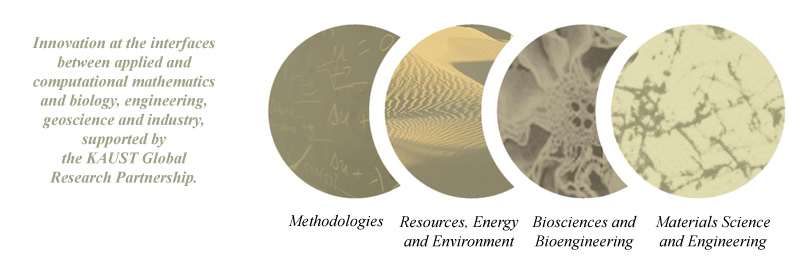
\includegraphics[width=\textwidth]{img/occam_4.jpg}

\end{frame}

%%% Frame

\begin{frame}\frametitle{Research -- Problem-driven themes}

Four interdisciplinary research areas:

\begin{overlayarea}{\textwidth}{0.3\textheight}
\begin{enumerate}

\item\alert<2>{Resources, Energy and Environment}\\
	\only<2>{{\tiny Lattice Boltzmann for CO$_2$ Sequestration; Oil Reservoir simulation; Desert landforms; Oilfield history matching.}}

\item\alert<3>{Biosciences and Bioengineering}\\
	\only<3>{{\tiny Crop growth in stressed environments; Tear film dynamics.}}

\item\alert<4>{Materials Science and Engineering}\\
	\only<4>{{\tiny Dislocations; Ionic surfactants; Electrochemistry.}}

\item\alert<5>{Mathematical and Computational Methodologies}\\
        \only<5>{{\tiny Numerical multiphysics; Design optimisation; Visualisation.}}

\end{enumerate}

\end{overlayarea}

%%% Frame

\end{frame}

\section{OCCAM}

\begin{frame}\frametitle{OCCAM}
\framesubtitle{What is it?}

\centerline{
\includegraphics[height=16mm]{img/image.png}}

\bigskip

\pause
Use \emph{focused teamwork}\\
\pause
with \emph{innovative} mathematical and computational methods\\
\pause
to help \emph{understand} pressing unsolved problems.

\bigskip

\end{frame}

%%% Frame

\section{What it offers}

\begin{frame}\frametitle{OCCAM}
\framesubtitle{What does it have to offer?}

\begin{itemize}

\item Network of experts in mathematical modelling.
\pause

\item Fresh look at the problems.\\
Ask the ``right'' questions $\to$ New approaches.
\pause

\item Recurrence of mathematics in different fields (Universality).\\
{\tiny (Port techniques from one field to another)}

\end{itemize}

\end{frame}

%%%%%%%%%%%%%%%%%%%%%%%%%%%%%%%%%%%%%%%%%%%%%%%%%%%%%%%%%%%%%%%%%%%%%%
%%                         THANK YOU FRAME
%%%%%%%%%%%%%%%%%%%%%%%%%%%%%%%%%%%%%%%%%%%%%%%%%%%%%%%%%%%%%%%%%%%%%%

\begin{frame}
\center

\vfill

{
\Huge%\color{occammedium}
\textbf{Thank you!}
}

\vfill

{\tiny
This presentation is based on work supported by

\smallskip


\includegraphics[height=12mm]{img/kaust_logo.jpg}
}

\end{frame}

\end{document}
